\documentclass[a4paper,11pt]{article}
\usepackage[T1]{fontenc}
\usepackage[utf8]{inputenc}
\usepackage{lmodern}
\usepackage[french]{babel} % or [english]
\usepackage{graphicx}
\usepackage{listings}
\usepackage{float}
\usepackage{placeins}
\usepackage{hyperref}
\usepackage{caption}
\usepackage{subcaption}
\usepackage{algorithm}
\usepackage{algpseudocode}

\usepackage{amsmath}
\usepackage{graphicx} % Required for inserting images

\begin{document}
\title{Projet Approche Objet}
\author{Abdoulaye Diallo, Théophyl Hoguet, Kea Horvath}
\date{Décembre 2023}
\begin{figure}
	\centering
	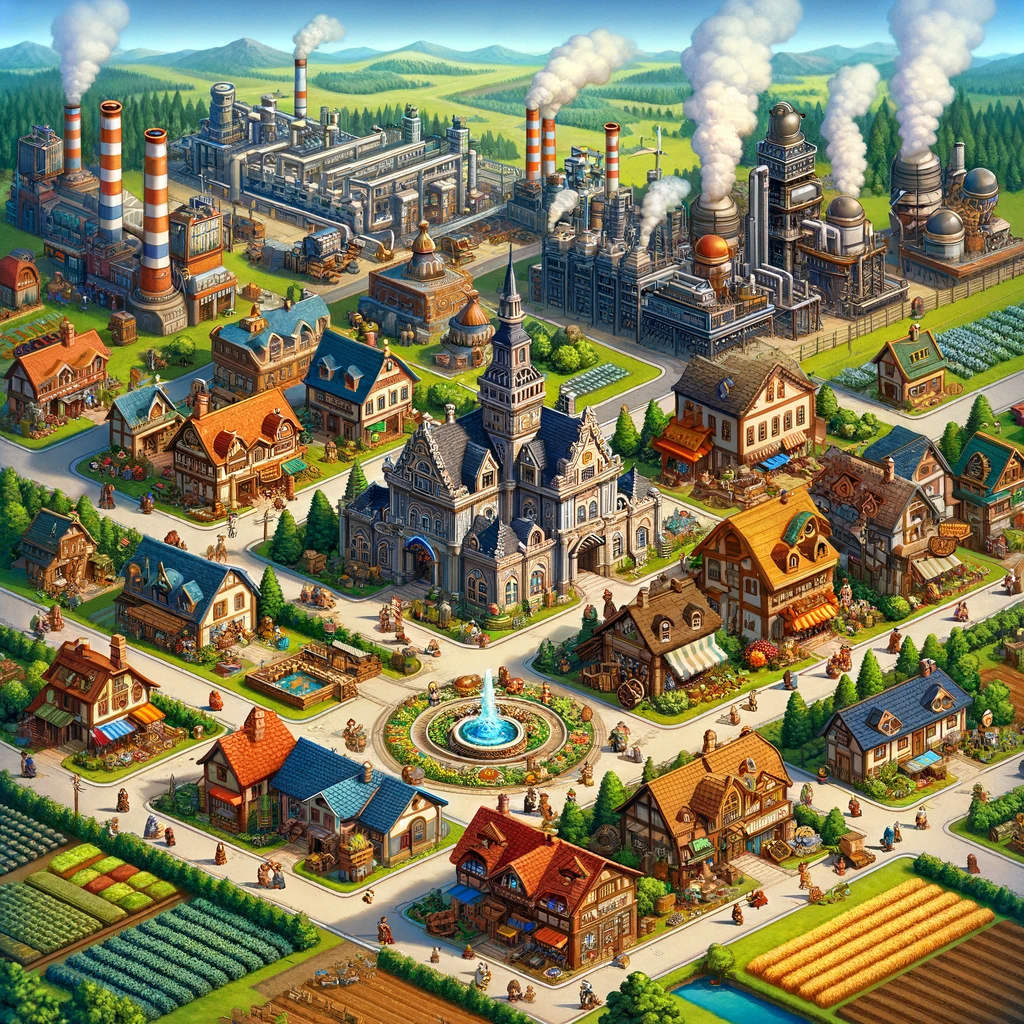
\includegraphics[width=0.75\linewidth]{Game.png}
	\label{fig:enter-label}
\end{figure}

\maketitle

\clearpage % Start a new page

\tableofcontents % Table of contents

\clearpage % Start a new page

\section{Analyse}
\subsection{Présentation}

\par
Pour ce projet de jeu de stratégie nous nous sommes mis à trois: Abdoulaye Diallo, Théophyl Hoguet et Kea Horvath. Le but du jeu est de permettre au joueur de gérer de manière stratégique une ville virtuelle, en prenant en charge la gestion des ressources, des habitants, des travailleurs et des bâtiments. L'objectif ultime est de faire prospérer l'économie de la ville aussi longtemps que possible. Le joueur a la possibilité d'utiliser des ressources pour construire de nouveaux bâtiments. Chaque bâtiment créé consomme une certaine quantité de ressource mais peut également en fabriquer. De plus, les habitants et les travailleurs consomment de la nourriture (une unité de \texttt{FOOD} par jour et par habitant). Le joueur doit prendre des décisions réfléchies pour maximiser la production, minimiser les pertes, et maintenir l'équilibre financier de la ville. Le joueur perd quand il n'y a plus nourriture (\texttt{FOOD}) pour nourrir sa population.

\subsection{Bâtiments}
Les bâtiments que nous avons inclus dans notre implémentation sont :

\begin{itemize}
	\item \textbf{Wooden Cabin:}
	      \begin{itemize}
		      \item Abrite: 4 habitants + 4 travailleurs minimum
		      \item Coûte: 1 GOLD + 1 WOOD
		      \item Prend 2 jours à construire
		      \item Produit: 6 WOOD + 8 FOOD
	      \end{itemize}

	\item \textbf{House:}
	      \begin{itemize}
		      \item Abrite: 8 habitants minimum
		      \item Coûte: 1 GOLD + 2 WOOD + 2 STONE
		      \item Prend 4 jours à construire
		      \item Produit: rien
	      \end{itemize}

	\item \textbf{Apartment Building:}
	      \begin{itemize}
		      \item Abrite: 32 habitants minimum
		      \item Coûte: 4 GOLD + 50 WOOD + 50 STONE
		      \item Prend 6 jours à construire
		      \item Produit: rien
	      \end{itemize}

	\item \textbf{Farm:}
	      \begin{itemize}
		      \item Abrite: 10 habitants + 5 travailleurs minimum
		      \item Coûte: 4 GOLD + 5 WOOD + 5 STONE
		      \item Prend 2 jours à construire
		      \item Produit: 10 FOOD
	      \end{itemize}

	\item \textbf{Quarry:}
	      \begin{itemize}
		      \item Abrite: 5 habitants + 15 travailleurs minimum
		      \item Coûte: 4 GOLD + 50 WOOD
		      \item Prend 2 jours à construire
		      \item Produit: 4 STONE + 4 IRON + 4 COAL + 2 GOLD
	      \end{itemize}

	\item \textbf{Lumber Mill:}
	      \begin{itemize}
		      \item Abrite: 10 travailleurs minimum
		      \item Coûte: 6 GOLD + 50 Wood + 50 Stone
		      \item Prend 4 jours à construire
		      \item Consomme: 4 WOOD
		      \item Produit: 4 LUMBER
	      \end{itemize}

	\item \textbf{Cement Plant:}
	      \begin{itemize}
		      \item Abrite: 10 travailleurs minimum
		      \item Coûte: 6 GOLD + 50 Wood + 50 Stone
		      \item Prend 4 jours à construire
		      \item Consomme: 4 COAL + 4 CEMENT
		      \item Produit: 4 CEMENT
	      \end{itemize}

	\item \textbf{Steel Mill:}
	      \begin{itemize}
		      \item Abrite: 20 travailleurs minimum
		      \item Coûte: 6 GOLD + 100 Wood + 50 Stone
		      \item Prend 6 jours à construire
		      \item Consomme: 2 COAL + 4 STEEL
		      \item Produit: 4 STEEL
	      \end{itemize}

	\item \textbf{Tool Factory:}
	      \begin{itemize}
		      \item Abrite: 12 travailleurs minimum
		      \item Coûte: 8 GOLD + 50 Wood + 50 Stone
		      \item Prend 8 jours à construire
		      \item Consomme: 4 COAL + 4 STEEL
		      \item Produit: 4 TOOL
	      \end{itemize}
\end{itemize}


\subsection{Comment jouer} % + Elements Clés :

\subsubsection{But du jeu:}
Le but du jeu est de maintenir une économie stable le plus longtemps possible sans que la nourriture ne vienne à manquer. Le joueur doit prendre garde à toujours avoir assez de ressources pour nourrir tout sa population.

\subsubsection{Début du jeu:}
Au début du jeu le joueur possède des ressources initiales et un ou deux bâtiments. Le joueur commence sans habitants ou travailleurs, il pourra ajouter autant d'habitants et/ou travailleurs que la capacité du bâtiment le permettra.

\subsubsection{Condition de perte:}
La partie se termine si la quantité de nourriture restante n'est pas suffisante pour tous les habitants et travailleurs de la ville. Donc la quantité de nourriture disponible représente la satisfaction de la population de la ville.

\subsubsection{Obtention/ Perte de ressources:}
Le joueur obtient des ressources chaque nouveau jour en fonction des bâtiments qui en produisent. La plupart des bâtiments produisent des ressources collectées en début de journée. Le joueur perd une quantité de nourriture proportionnelle au nombre d'habitants et de travailleurs dans la ville. Il a également la possibilité d'utiliser ces ressources pour construire des bâtiments.

Dans notre jeu, il est possible d'améliorer les bâtiments pour un certain coût, en fonction du bâtiment et de son niveau. A chaque niveau le coût d'amélioration du bâtiment augmente mais ses productions aussi.

\subsubsection{Construction/Destruction de bâtiments:}
Pour construire un bâtiment, le joueur doit utiliser ses ressources. Chaque bâtiment a un coût en or et en matériaux qui lui est propre. De plus, chaque bâtiment a une durée de construction avant d'être disponible et de produire ses ressources.
A l'opposé, la destruction d'un bâtiment se fait immédiatement. Le joueur récupère alors la moitié des ressources qu'il a utilisé pour construire le bâtiment, on ignore les améliorations faites au bâtiment.

\subsubsection{Gestion du temps :}
Dans notre jeu une journée dure une seconde et demi. Ceci pourrait sembler rapide mais le joueur a l'option de mettre le jeu en pause pour prendre ses décisions.

\subsubsection{Score :}
Nous avons aussi décidé de mettre en place un compteur de score qui évolue en fonction du nombre de ressource et d'un multiplicateur de ressource.

\subsubsection{Interface Utilisateur:}
Nous avons choisi d'implémenter une interface graphique pour notre jeu. La ville est représentée par un grid de plusieurs cellules, qui seront les emplacements des bâtiments construits.
Pour construire un bâtiment, le joueur clique gauche sur un bâtiment et sur une cellule libre.

\clearpage

\section{Conception}
\subsection{\text{DDD} + Architecture de nos classes} %Structure du projet
\subsubsection*{} %justifier les choix de mise en oeuvre du DDD
Pour la partie conception de notre projet nous avons décidé d'utiliser le \text{DDD(Domain Driven Design)}. Le \text{DDD} est le design pattern le plus utile pour un jeu avec une division de l'application en plusieurs couches. Ce qui simplifie grandement la conception et la maintenance du projet.

% repond à la partie  donnera l’architecture de vos classes, les differents mod`eles Design Patterns que vous aurez ´eventuellement utilis´es et/ou les concepts DDD si vous les avez mis en oeuvre dans votre code; vous ne trouvez pas ?
Dans le cadre du \text{DDD}, nous identifions plusieurs \texttt{Value Objects} importants pour la représentation des concepts clés de notre jeu. Parmi eux, nous avons les objets tels que \texttt{BuildingType} pour décrire les différents types de bâtiments, ainsi que des objets relatifs aux ressources tels que \texttt{Resource}, \texttt{ResourceType}, \texttt{ResourceList}, et \texttt{ResourceAmount}. Nous incorporons également des objets tels que \texttt{Grid} pour la gestion de l'espace dans le jeu, ainsi que des objets liés aux besoins tels que \texttt{Needs}, et \texttt{Production}, \texttt{Consumption}, et \texttt{ConstructionNeeds} qui étendent \texttt{Needs}.

Dans notre jeu, nous avons \texttt{Building} comme une \texttt{Entity} principale, représentant les bâtiments dans notre ville. Enfin, l'\texttt{Aggregate} \texttt{Manager} est présente pour englober et coordonner les différents éléments du jeu, assurant ainsi une gestion efficace et une cohérence globale. Notre \texttt{Manager} nous permet de manipuler tout les aspects de notre jeu grâce aux \texttt{Value Objects} de nos différents bâtiments.

\subsubsection*{}
Les classes qui manipulent le plus notre jeu sont \texttt{Manager} et \texttt{Building}, elles permettent de :
\begin{itemize}
	\item Construire/ Détruire des bâtiments : \texttt{buildBuilding()} / \texttt{destroyBuilding()} dans \texttt{Manager}
	\item Ajouter / Supprimer des habitants/travailleurs: \texttt{addInhabitantsToBuilding()} / \texttt{removeInhabitantsFromBuilding()} dans \texttt{Manager}
	\item Mettre le jeu en pause ou le terminer si le joueur n'a plus de nourriture: \texttt{}
	\item Mettre à jour toutes ressources du jeu en fonction des consommations et des productions : \texttt{update()} dans \texttt{Manager}
	\item Améliorer des bâtiments : \texttt{upgradeBuilding()} dans \texttt{Manager}
\end{itemize}

\clearpage

\subsection{Début d'une partie}
\par Au début du jeu, les joueurs peuvent choisir l'un des trois niveaux de difficulté proposés : \texttt{Easy}, \texttt{Normal}, ou \texttt{Hard}. Ce choix est représenté par la classe enum \texttt{GameStarter}. Chaque niveau de difficulté est associé à un ensemble de ressources et de bâtiments initiaux. Par exemple, le niveau \texttt{Easy} offre plus de ressources que les niveaux \texttt{Normal} et \texttt{Hard}. La classe \texttt{GameStarter} stocke ces informations. Si le joueur choisit le niveau de difficulté \texttt{Easy}, la classe \texttt{Main} utilise les informations définies dans l'énumération \texttt{GameStarter.EASY} pour initialiser la partie. Ces informations déterminent le nombre d'habitants, de travailleurs, les ressources de départ et les bâtiments avec lesquelles le joueur commence. L'utilisation d'un énumération permet de gérer facilement les différentes configurations de jeu.

\par Une fois le niveau choisi le joueur peut créer des bâtiments pour gagner plus de ressources, ou rajouter des habitants ou travailleurs dans les bâtiments. Par exemple, si le joueur choisit de construire un bâtiment \texttt{HOUSE}, \texttt{App} va appeler sa méthode \texttt{buildBuilding} qui va appeler \texttt{buildBuilding} de \texttt{Manager}. \texttt{Manager} va vérifier si l'emplacement choisi pour la construction du bâtiment est libre. Si elle l'est le bâtiment sera construit, sinon une \texttt{exception} sera lancé. Le joueur peut construire autant de bâtiments qu'il le souhaite tant qu'il a les ressources pour ces constructions. Une fois les constructions faites le joueur peut ajouter des habitants ou travailleurs qui consommeront des ressources. Si le joueur a assez de ressources il peut améliorer ses bâtiments déjà construits. Ceci appelle \texttt{isBuildingUpgradeable} de \texttt{Manager} qui appelle \texttt{canUpgrade} de \texttt{Building} pour vérifier les ressources du joueur. Si \texttt{canUpgrade} retourne \texttt{true} alors \texttt{upgrade} de \texttt{Building} est lancé pour améliorer le bâtiment. Une fois amélioré le bâtiment produit et consomme plus de ressources. Le joueur pourra continuer à construire et/ou modifier ses bâtiments ou encore augmenter sa population tant qu'il possède des ressources.

\clearpage

\subsection{Options de notre jeu}
\begin{itemize}
	\item \textbf{Play / Pause : } Notre jeu offre au joueur la possibilité de mettre le jeu en pause et de le reprendre ensuite à l'aide d'un bouton. Cela donne un temps de reflection au joueur.

	\item \textbf{Construction d'un bâtiment : } Le joueur choisi le bâtiment qu'il souhaite construire, et dont il a les ressources. Il choisi ensuite une cellule libre dans laquelle cet bâtiment sera placé.

	\item \textbf{Amélioration des bâtiments : } Lorsque le joueur souhaite améliorer un bâtiment
	      \begin{itemize}
		      \item Chaque amélioration augmente les coûts de construction de 25\% pour la prochaine amélioration.
		      \item Chaque amélioration double la consommation et la production du bâtiment.
		      \item Chaque amélioration multiplie le nombre d'habitants et/ou de travailleurs par 1.5.
	      \end{itemize}
	\item \textbf{Destruction d'un bâtiment : } Lorsque le joueur souhaite détruire un bâtiment, il effectue un clic droit sur la cellule du bâtiment, un menu se déroule, et il peut ensuite cliquer sur "Destroy."

	\item \textbf{Ajout / Suppression d'habitants / de travailleurs : } Un clic-doit sur un bâtiment déroule un menu avec les options relatives aux habitants/travailleurs du bâtiment.

	\item \textbf{Sauvegarde d'une partie dans un fichier : } À tout moment pendant sa partie, le joueur peut mettre le jeu en pause et sauvegarder dans un fichier.

	\item \textbf{Chargement d'une partie à partir d'un fichier : } Le joueur a le choix de créer une nouvelle partie ou de jouer à partir d'une partie précédemment sauvegardée.
\end{itemize}


\subsection{Interface graphique}
Pour l'interface utilisateur nous avons décidé de créer une interface graphique avec javafx.


\subsubsection{Voici les fonctionnalités de notre interface graphique : }
\begin{itemize}
	\item \text{Bouton Play / Pause}
	\item \text{Construction de bâtiment : } faire un clic-gauche sur un bâtiment que l'on veut créer puis faire un clic-gauche sur une cellule libre du grid.
	\item \text{Modifications de bâtiments : } faire un clic-droit sur un bâtiment déroule un menu de choix possibles.
	      \begin{itemize}
		      \item Destruction de bâtiment : choisir "\texttt{Destroy}"
		      \item Amélioration de bâtiment : choisir "\texttt{Upgrade}" %choisir "Is Upgradeable ?", si la fenêtre dit "oui" alors choisir 
		      \item Ajouter des habitants : choisir "\texttt{Add Inhabitants}"
		      \item Supprimer des habitants : choisir "\texttt{Remove Inhabitants}"
		      \item Ajouter des travailleurs : choisir "\texttt{Add Workers}"
		      \item Supprimer des travailleurs : choisir "\texttt{Remove Workers}"
	      \end{itemize}
	\item \text{Affichage des informations d'un bâtiment : } faire un clic-gauche sur un bâtiment déjà construit
\end{itemize}


\clearpage

\section{Conclusion}
En conclusion, durant ce projet nous avons pu voir les points délicats de la création de jeu de stratégie et les décisions qui poussent à incorporer un aspect plutôt qu'un autre.

L'utilisation du \text{DDD} nous a permis de travailler de manière efficace et de diviser le projet en plusieurs sous-domaines qui ont rendu le tout très cohérent.
Les \text{Value Objects}, \text{Entities}, et \text{Aggregates} définis par le \text{DDD} ont été essentiels pour représenter efficacement les concepts clés du jeu, tels que les types de bâtiments et les ressources.

En plus de la conception, notre ajout d'une interface graphique rend notre jeu plus agréable à jouer. Nous pensons que les ajouts et modifications de bâtiments se font facilement.

En fin de compte, ce projet nous a permis de consolider nos compétences en programmation orientée objet, la réflexion derrière la conception de jeu et la collaboration en équipe. Bien que le jeu soit assez simple en termes d'options, nous considérons que nous avons accompli les grandes attentes de notre jeu.

\section{Annexe-}
\begin{table}[ht]
	\centering
	\begin{subtable}{.3\linewidth}
		\centering
		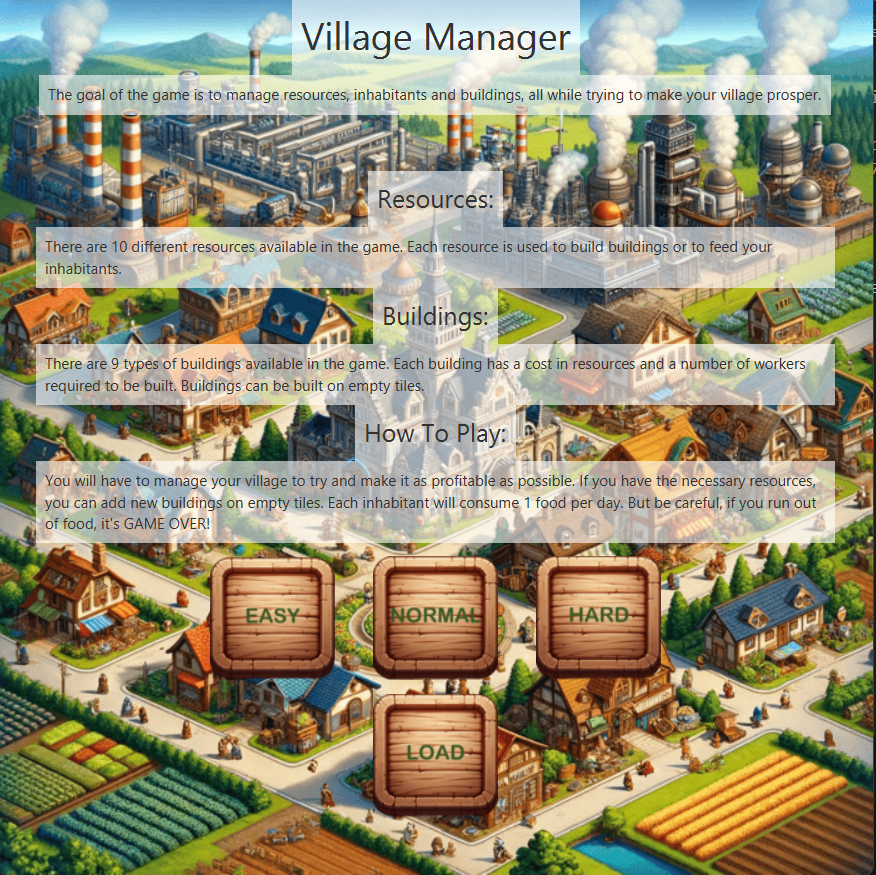
\includegraphics[width=1\linewidth]{startPage.png}
		\caption{Lancement d'une partie}
		\label{subfig:image1}
	\end{subtable}%
	\hfill
	\begin{subtable}{.3\linewidth}
		\centering
		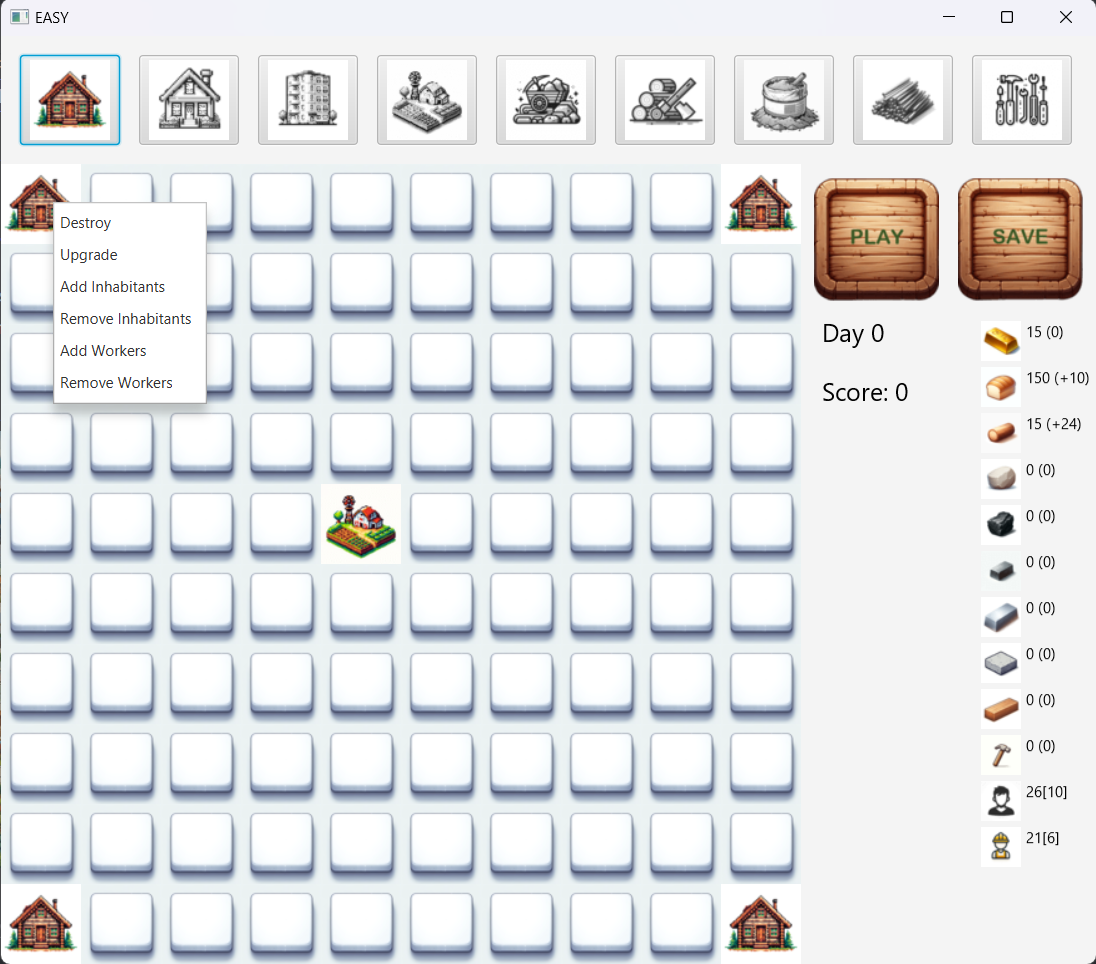
\includegraphics[width=1\linewidth]{mid_game.png}
		\caption{En cours de partie}
		\label{subfig:image2}
	\end{subtable}%
	\hfill
	\begin{subtable}{.3\linewidth}
		\centering
		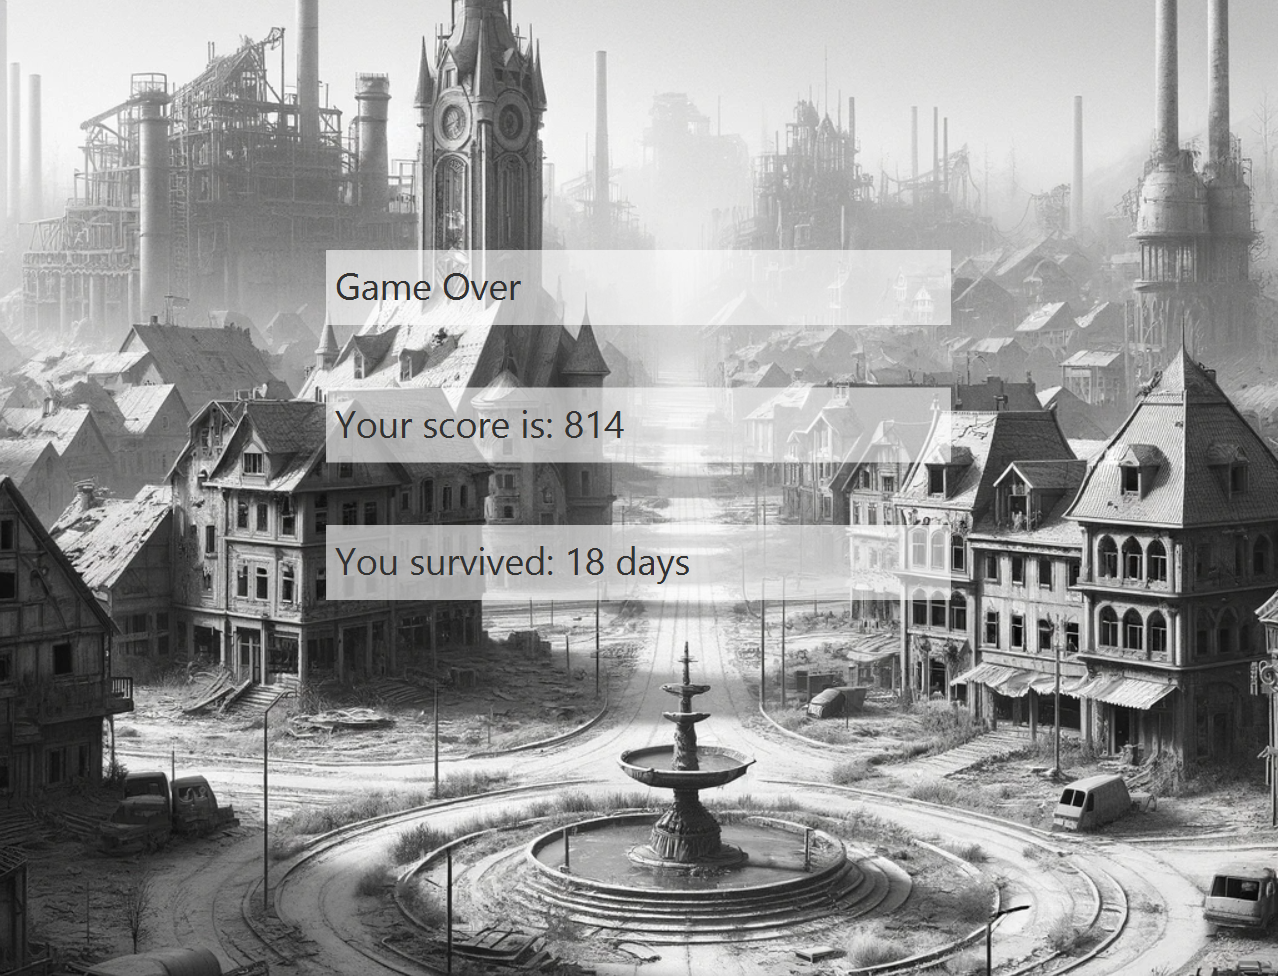
\includegraphics[width=1\linewidth]{game_over.png}
		\caption{Fin de partie}
		\label{subfig:image3}
	\end{subtable}
	\begin{subtable}{.3\linewidth}
		\centering
		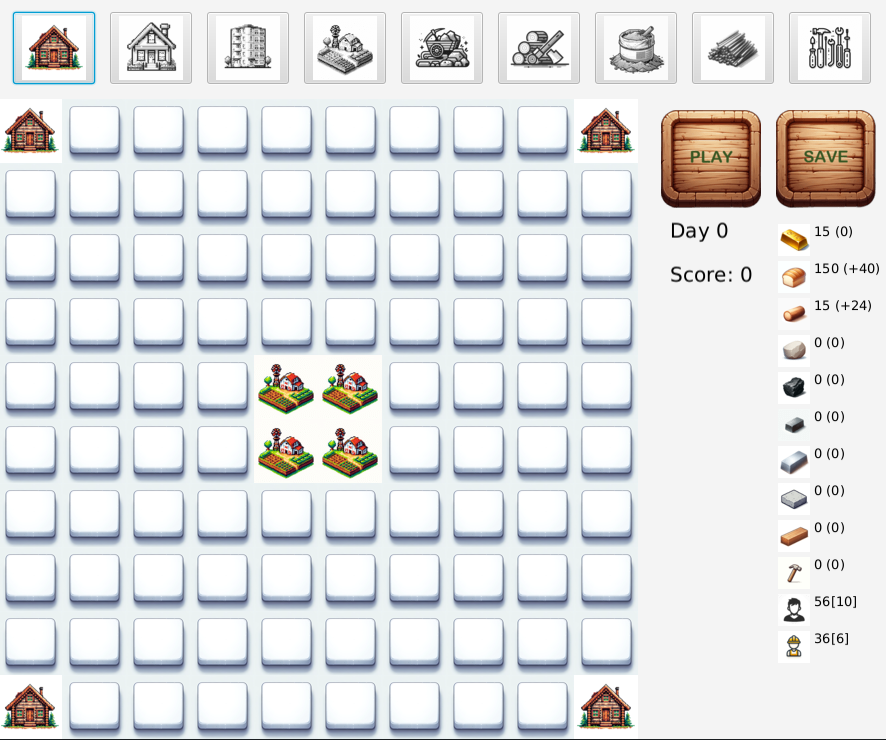
\includegraphics[width=1\linewidth]{mid_game_2.png}
		\caption{Fin de partie}
		\label{subfig:image4}
	\end{subtable}
	\caption{Images de notre jeu}
	\label{fig:overall_label}
\end{table}

\end{document}
